% ===========================================================================
% Chatbots
% Traduit et adapté de :
%   https://www.bootstrapworld.org/materials/fall2026/en-us/lessons/stat-lang-models-chatbots/
% Licence : Creative Commons 4.0 Unported (Bootstrap Community)
% ===========================================================================

\documentclass[12pt,a4paper]{article}

% ---------- Packages ----------
\usepackage[utf8]{inputenc}
\usepackage[T1]{fontenc}
\usepackage{libertine}
\usepackage{microtype}
\usepackage[french]{babel}
\usepackage{graphicx}
\usepackage{float}
\usepackage{hyperref}
\usepackage{geometry}
\usepackage{enumitem}
\usepackage{tabularx}
\usepackage{xcolor}
\usepackage{colortbl}
\usepackage[raster]{tcolorbox}
\usepackage{booktabs}
\usepackage{fancyhdr}
\usepackage{titlesec}
\usepackage{amsmath}
\usepackage{amssymb}

% ---------- Mise en page ----------
\geometry{margin=2.5cm, headheight=15pt, footskip=30pt}
\fancyhf{}
\fancyhead[L]{\textbf{Chatbots}}
\fancyhead[R]{\thepage}
\fancyfoot[C]{Bootstrap Community — CC BY 4.0}
\renewcommand{\headrulewidth}{0.4pt}
\pagestyle{fancy}

% ---------- Couleurs ----------
\definecolor{bsblue}{RGB}{41,128,185}
\definecolor{bsgreen}{RGB}{39,174,96}
\definecolor{bsorange}{RGB}{230,126,34}
\definecolor{bsgray}{RGB}{149,165,166}
\definecolor{codebg}{RGB}{245,247,250}

% ---------- Styles de sections ----------
\titleformat{\section}[hang]{\Huge\bfseries\color{bsblue}}{}{0pt}{}[\vspace{-0.5em}\rule{\textwidth}{2pt}]
\titleformat{\subsection}[hang]{\Large\bfseries\color{bsblue!80!black}}{}{0pt}{}
\titleformat{\subsubsection}[hang]{\large\bfseries\color{bsgreen!60!black}}{}{0pt}{}

% ---------- Environnements personnalisés ----------
\newtcolorbox{overviewbox}{
  colback=bsblue!5!white, colframe=bsblue!60!white,
  fonttitle=\bfseries, title=Objectif de la section,
  left=1em, right=1em, top=0.5em, bottom=0.5em
}
\newtcolorbox{activitybox}{
  colback=bsgreen!5!white, colframe=bsgreen!60!white,
  fonttitle=\bfseries, title=Activité,
  left=1em, right=1em, top=0.5em, bottom=0.5em
}
\newtcolorbox{thinkbox}{
  colback=bsorange!5!white, colframe=bsorange!60!white,
  fonttitle=\bfseries, title=Réflexion,
  left=1em, right=1em, top=0.5em, bottom=0.5em
}
\newtcolorbox{keypointbox}{
  colback=bsgray!10!white, colframe=bsgray!50!white,
  fonttitle=\bfseries, title=Point clé,
  left=1em, right=1em, top=0.5em, bottom=0.5em
}
\newtcolorbox{instructornotes}{
  colback=yellow!10!white, colframe=yellow!80!black,
  fonttitle=\bfseries, title=Notes pour l'enseignant·e,
  left=1em, right=1em, top=0.5em, bottom=0.5em
}

% ---------- Commandes pratiques ----------
\newcommand{\img}[3]{%
  \begin{figure}[H]
    \centering
    \includegraphics[#2]{#1}
    \caption{#3}
    \label{fig:#1}
  \end{figure}
}
% Icônes de Soekia (petites images en ligne)
\newcommand{\soekiaicon}[2]{\includegraphics[height=#2]{#1}}

% ---------- Informations du document ----------
\title{%
  \vspace{-2cm}
  {\Huge\bfseries Chatbots}\\[0.5em]
  {\large Modèles de langue statistiques, température et langages artificiels}\\[1em]
  {\normalsize Traduit et adapté depuis \href{https://www.bootstrapworld.org/materials/fall2026/en-us/lessons/stat-lang-models-chatbots/}{Bootstrap World} (Fall 2026)}\\
  {\normalsize Adapté au contexte francophone — outil Soekia en français}\\[0.5em]
  {\normalsize Licence Creative Commons 4.0 International}
}
\date{}
\author{}

\begin{document}

\maketitle
\thispagestyle{empty}

\vspace{2cm}
\begin{center}
  \textit{Ces supports ont été développés en partie grâce au soutien de la National Science Foundation\\
  (bourses 1042210, 1535276, 1648684, 1738598, 2031479 et 1501927).}
\end{center}

\newpage
\tableofcontents
\newpage

% ===========================================================================
% SECTION 1 : RENCONTRE AVEC SOEKIA
% ===========================================================================
\section{Rencontre avec Soekia}

\begin{overviewbox}
  Les élèves découvrent Soekia, un modèle de langue statistique conçu pour l'apprentissage, et explorent certaines des nuances de ce type de modèle.
\end{overviewbox}

% ---------- Launch ----------
\subsection{Lancement}

Vous avez déjà appris comment les modèles de langue statistiques reposent sur la probabilité pour générer du texte, et vous avez construit votre propre modèle de langue à partir de la chanson enfantine \emph{«~Une vieille dame avala une mouche~»} dans la leçon \emph{Modèles génératifs}.

Dans cette leçon, vous allez explorer \textbf{Soekia}, un outil d'apprentissage spécialement conçu pour la génération de texte. Soekia nous offre un exemple de \textbf{traitement du langage naturel} (\emph{Natural Language Processing}).

\begin{keypointbox}
  \textbf{Pour commencer}
  \begin{itemize}
    \item Ouvrez une fenêtre de navigateur et assurez-vous qu'elle occupe toute la largeur de votre écran.
    \item Allez sur l'\textbf{outil Soekia en français}~: \url{https://www.soekia.ch/GPT/?lang=FR}
    \item Le panneau \textbf{bleu} qui occupe la plus grande partie de l'écran est l'endroit où la génération de texte a lieu. C'est le niveau généralement visible pour l'utilisateur·trice d'un chatbot.
    \item Nous allons demander à Soekia de générer un conte de fées en cliquant sur le bouton de génération~: \soekiaicon{images/c4b181ce83ec98ed.png}{1.1em}.
    \item Suivez du regard et lisez le texte jusqu'à ce que Soekia finisse d'écrire.
  \end{itemize}
\end{keypointbox}

\begin{activitybox}
  Complétez la première section de \emph{Rencontrer Soekia~!}.
\end{activitybox}

\begin{thinkbox}
  \textbf{Que remarquez-vous~?}
  \begin{itemize}
    \item Un nouveau mot apparaît environ une fois par seconde.
    \item Différents mots apparaissent dans différentes couleurs.
    \item Le conte de fées sonne un peu étrange.
    \item Nous pouvons mettre en pause, accélérer, ou ajouter un mot à la fois en utilisant les commandes de lecture sous la fenêtre de texte.
    \item Nous pouvons demander à Soekia d'écrire un autre paragraphe en cliquant sur \soekiaicon{images/b312953ac30ff5de.png}{1.1em}~«~Reprendre automatiquement~».
    \item Nous pouvons manuellement sélectionner le mot suivant dans une liste si nous le voulons.
    \item Pour écrire une nouvelle histoire, nous pouvons cliquer sur l'icône de réinitialisation pour supprimer ce qui a été généré.
    \item Nous pouvons copier le texte généré dans notre presse-papiers en utilisant l'icône \soekiaicon{images/11d015d04de6390c.png}{1.1em}.
    \item Nous pouvons activer ou désactiver le code couleur des mots en cliquant sur l'icône «~œil~».
    \item Nous pouvons passer de la génération de texte continue au mode \soekiaicon{images/e8927b4ad6886e51.png}{1.1em}~«~mot à mot~» ou au mode «~rapide~».
  \end{itemize}
\end{thinkbox}

\begin{thinkbox}
  \textbf{Que vous demandez-vous~?}
  \begin{itemize}
    \item Pourquoi l'histoire sonne-t-elle si bizarre~?
    \item Soekia racontera-t-il une histoire différente chaque fois que je lui en demande une~?
    \item ChatGPT utilise-t-il le même algorithme que Soekia~?
    \item Pourquoi les mots sont-ils surlignés de différentes couleurs~?
  \end{itemize}
\end{thinkbox}

\begin{activitybox}
  Survolez avec la souris un ou deux des mots surlignés dans le conte de fées. Qu'apparaît-il~?
  \begin{itemize}
    \item Si les mots de votre conte ne sont pas déjà surlignés de différentes couleurs (verts, violets, etc.), cliquez sur l'icône «~œil~» sous le texte généré.
    \item Chaque couleur correspond à un \textbf{document} différent~; les documents sont étiquetés A, B, C, etc.
  \end{itemize}
\end{activitybox}

% ---------- Investigate ----------
\subsection{Exploration~: regarder derrière le rideau}

Il est temps de jeter un coup d'œil derrière le rideau pour voir d'où vient le conte que vous avez lu~!

\begin{keypointbox}
  Cliquez sur le bouton «~REGARDER À L'INTÉRIEUR~» (\emph{LOOK INSIDE}) dans le coin supérieur droit de Soekia.
\end{keypointbox}

Maintenant, en plus du panneau bleu de génération de texte, nous voyons trois panneaux supplémentaires~: \textbf{mots suggérés}, \textbf{n-grammes}, et \textbf{documents}.

\img{images/fcba97f8c6eb32c0.png}{width=1.0\textwidth}{Capture d'écran des quatre panneaux de Soekia~: génération de texte (bleu), mots suggérés, n-grammes, et documents.}

Il y a beaucoup de choses à découvrir dans chaque panneau~!

\subsubsection{Le panneau Documents}

\begin{activitybox}
  Commençons par le panneau \textbf{Documents}.
  \begin{itemize}
    \item Tournez-vous vers \emph{Rencontrer Soekia~!} et complétez la page avec votre voisin·e.
  \end{itemize}
\end{activitybox}

\begin{thinkbox}
  \textbf{Qu'avez-vous remarqué à propos du panneau \emph{Documents}~?}
  \begin{itemize}
    \item Il y a 12~documents.
    \item Chaque document est d'une couleur différente.
    \item Les couleurs correspondent à celles qui apparaissent (en surlignant les mots) dans le panneau \emph{Génération de texte}.
    \item Si je clique sur les icônes en haut à droite, je peux changer le corpus d'entraînement.
    \item Si je change l'invite dans le panneau \emph{Génération de texte}, les lignes vertes en bas des documents changent. Ces lignes indiquent à quel point le libellé de l'invite correspond au texte du document.
  \end{itemize}

  \textbf{Que vous demandez-vous à propos du panneau \emph{Documents}~?}
  \begin{itemize}
    \item Puis-je changer ces documents pour d'autres~?
    \item Pourquoi n'ai-je pas entendu parler de certains de ces contes de fées~?
    \item Quelle est la relation entre ce panneau \emph{Documents} et le panneau \emph{N-grammes} à côté~?
  \end{itemize}
\end{thinkbox}

\begin{instructornotes}
  Invitez les élèves à partager leurs découvertes. Certain·es élèves découvriront peut-être qu'ils·elles peuvent changer le corpus d'entraînement pour que les documents incluent non pas des contes de fées mais des parties de tic-tac-toe, des compositions musicales, et des parties d'échecs~! Dans la section suivante de la leçon, les élèves exploreront ces autres collections de documents plus en profondeur.
\end{instructornotes}

\subsubsection{Le panneau N-grammes}

\begin{keypointbox}
  Avant de commencer à explorer les autres panneaux, nous voulons trouver une collection de documents plus petite et plus courte.

  \begin{itemize}
    \item Allez dans le menu déroulant des collections \soekiaicon{images/c4b181ce83ec98ed.png}{1.1em} et sélectionnez la collection \emph{Intelligent Monkeys~?}
    \item Une fois la collection ouverte, regardez le panneau \emph{N-grammes}. Par défaut, vous devriez voir~3 sélectionné en haut, ce qui signifie que tous les trigrammes possibles de la collection seront affichés, triés du plus fréquent au moins fréquent.
  \end{itemize}
\end{keypointbox}

\begin{activitybox}
  Tournez-vous vers \emph{Rencontrer Soekia~! (n-grammes)} et complétez la page avec votre voisin·e.
\end{activitybox}

\begin{instructornotes}
  Si vous terminez avant que nous soyons prêt·es à discuter en classe, voyez si vous pouvez prédire les 5~premiers mots que Soekia produirait à partir de la collection météo. \emph{Note~: quand vous changez de collection, la température se réinitialise automatiquement à 60, donc vous devrez la remettre sur~bas.}
\end{instructornotes}

\begin{keypointbox}
  Vous venez d'apprendre comment Soekia parcourt les différentes listes du panneau \emph{N-grammes} pour générer le mot suivant dans le champ de texte quand la température est réglée sur~bas. Vous avez aussi découvert que toutes les listes ne sont pas des «~n-grammes valides~» d'emblée.
\end{keypointbox}

\begin{thinkbox}
  \textbf{Pour prédire le mot suivant, quand Soekia choisira-t-il un mot dans la liste des unigrammes~?}
  \begin{itemize}
    \item Pour le premier mot. Et pour tout autre mot, quand il ne trouve pas de correspondance pour un n-gramme plus grand qui utilise les mots précédents.
  \end{itemize}

  \textbf{Si les quatre premiers mots dans le champ de génération de texte étaient «~Il était une fois~», que chercherait Soekia dans les onglets \emph{N-grammes} pour choisir le mot suivant~?}
  \begin{itemize}
    \item D'abord, il chercherait le 5-gramme le plus fréquent qui commence par «~Il était une fois~».
    \item S'il n'y en avait pas, il chercherait le 4-gramme le plus fréquent qui commence par «~était une fois~».
    \item S'il n'y en avait pas, il chercherait le trigramme le plus fréquent qui commence par «~une fois~».
    \item S'il n'y en avait pas, il chercherait le bigramme le plus fréquent qui commence par «~fois~».
    \item S'il n'y en avait pas, il chercherait l'unigramme le plus fréquent suivant.
  \end{itemize}

  \textbf{Qu'avez-vous remarqué d'autre à propos du panneau \emph{N-grammes}~?}
  \begin{itemize}
    \item Tous les n-grammes proviennent directement des documents.
    \item Je peux trier les n-grammes soit alphabétiquement, soit par fréquence.
    \item Soekia interprète les signes de ponctuation comme des mots.
    \item Je peux dire à Soekia de produire des unigrammes, bigrammes, trigrammes, etc.
    \item Soekia calcule la fréquence de chaque n-gramme, tout comme nous l'avons fait à partir du corpus \emph{«~Une vieille dame avala une mouche~»} dans la leçon \emph{Modèles génératifs}.
  \end{itemize}

  \textbf{Que vous demandez-vous à propos du panneau \emph{N-grammes}~?}
  \begin{itemize}
    \item Pourquoi Soekia interprète-t-il la ponctuation comme un mot~?
    \item Comment Soekia décide-t-il quel n-gramme il va utiliser dans le conte de fées~?
  \end{itemize}
\end{thinkbox}

\subsubsection{La température}

Nous venons de voir comment Soekia choisit le mot suivant avec la température réglée sur~bas, mais qu'est-ce que cela signifie~?

\begin{keypointbox}
  \textbf{La température}

  Quand la température est \textbf{zéro}, nous suivons un algorithme qui retourne très rigoureusement les n-grammes les plus fréquents du corpus. Des températures plus élevées introduisent un certain degré d'\textbf{aléatoire}. En fait, quand la température est de~60, cela signifie qu'il y a 60~\% de chances que nous regardions en dehors du premier ensemble (les n-grammes les plus fréquents).
\end{keypointbox}

\begin{keypointbox}
  \textbf{Pourquoi voudrions-nous introduire de l'aléatoire dans notre génération de texte~?}

  Il y a plusieurs raisons~:
  \begin{itemize}
    \item Quand nous avons demandé à Soekia de générer du texte avec zéro aléatoire à partir de la collection \emph{Intelligent Monkeys~?}, rester sur les n-grammes les plus fréquents nous a piégés dans une boucle répétitive de trois mots~!
    \item Nous ne voulons peut-être pas que la même invite génère exactement le même contenu à chaque fois.
    \item Nous voulons peut-être générer du texte qui nous pousse à penser de façon créative, au-delà des limites de la boîte dans laquelle nos idées sont enfermées.
  \end{itemize}
\end{keypointbox}

\subsubsection{Les «~hallucinations~» de l'IA}

\begin{keypointbox}
  \textbf{Les «~hallucinations~» de l'IA}

  Quand une IA générative produit du texte, elle génère souvent des informations incorrectes ou trompeuses. C'est communément appelé une «~hallucination~» de l'IA.

  Certain·es expert·es n'aiment pas ce terme et encouragent à cesser de l'utiliser. Ces expert·es affirment que \emph{toute} la production est «~hallucinatoire~». Une partie de celle-ci se trouve correspondre à la réalité…~et une partie non.

  \vspace{0.3em}
  \emph{Le même processus} qui génère du texte «~hallucinatoire~» génère \emph{aussi} le texte «~non hallucinatoire~». Cette vérité nous aide à comprendre \emph{pourquoi} il est si difficile de \textbf{réparer} le problème de l'«~hallucination~».

  \vspace{0.3em}
  Ce terme attribue aussi une intention et une conscience à l'IA, lui donnant des qualités humaines alors qu'elle exécute simplement un programme exactement comme il est prévu qu'il le fasse.
\end{keypointbox}

\begin{instructornotes}
  Pensez-vous que vos élèves aimeraient en apprendre davantage sur des exemples spécifiques d'hallucinations de l'IA~? Si oui, imprimez et distribuez le polycopié optionnel \emph{Famous AI Disasters} (\texttt{famous-ai-disasters.pdf}).
\end{instructornotes}

\begin{activitybox}
  Retournez à Soekia et ouvrez la collection météo.
  \begin{itemize}
    \item Dans le panneau \emph{Mots suggérés}, cliquez sur «~Personnaliser la température / le nombre de suggestions~» et réglez la température sur~bas.
    \item Puis cliquez sur le bouton de génération dans le panneau \emph{Générer du texte} et regardez le texte être généré à la fois là et dans le panneau \emph{Mots suggérés}.
    \item Répétez le processus pour d'autres réglages de température, en remarquant comment la langue change.
  \end{itemize}
\end{activitybox}

\begin{thinkbox}
  \textbf{Qu'avez-vous remarqué~?}
  \begin{itemize}
    \item Le panneau \emph{Mots suggérés} se met à jour automatiquement à mesure que Soekia génère du texte.
    \item Soekia suggère souvent un 5-gramme et les n-grammes plus courts contenus dans ce 5-gramme (par exemple, «~le vent dans les arbres~», «~vent dans les arbres~», «~dans les arbres~» et «~arbres~»).
  \end{itemize}
\end{thinkbox}

% ---------- Synthesize ----------
\subsection{Synthèse}

\begin{thinkbox}
  \textbf{Décrivez avec vos propres mots ce qui se passe dans chacun des panneaux internes de Soekia.}
  \begin{itemize}
    \item Le panneau \emph{Documents} contient le corpus d'entraînement.
    \item Soekia traite les documents et produit une liste de tous les n-grammes possibles (pour un $n$ donné) dans le panneau \emph{N-grammes}.
    \item Dans le panneau \emph{Mots suggérés}, Soekia propose des complétions possibles pour différentes entrées.
    \item L'utilisateur·trice peut régler la température pour choisir des suggestions de mots fréquents (température basse) ou pour suggérer des mots plus aléatoirement (température haute).
    \item Dans le panneau \emph{Génération de texte}, la sortie apparaît automatiquement ou l'utilisateur·trice peut choisir de sélectionner chaque mot dans une liste de suggestions.
  \end{itemize}
\end{thinkbox}

\begin{thinkbox}
  L'apprentissage supervisé comprend trois étapes~: la \emph{démonstration} du processus d'apprentissage, l'\emph{abstraction de fonction}, et l'\emph{utilisation} de la fonction. Décrivez ce que chaque étape inclut pour l'apprentissage supervisé d'un modèle de langue.
  \begin{itemize}
    \item \textbf{Démonstration~:} pour les modèles de langue statistiques, la phase de démonstration est moins évidente que dans les autres cas que nous avons étudiés (voitures autonomes et arbres de décision). Essentiellement, un·e superviseur·e humain·e est nécessaire pour sélectionner les documents qui forment le corpus d'entraînement. La démonstration selon laquelle «~étant donné un n-gramme, la complétion est \_\_~» est implicite, pas explicite. Il serait d'une ampleur vertigineuse pour un humain de devoir démontrer chacune de ces complétions~! Au lieu de cela, la «~supervision~» vient des probabilités que l'ordinateur a calculées à partir du corpus.
    \item \textbf{Abstraction de fonction~:} un modèle de langue statistique attribue des probabilités à différentes séquences de mots, indiquant leur probabilité d'apparition en fonction des mots (ou n-grammes) précédents.
    \item \textbf{Utilisation~:} l'utilisation de la fonction implique de générer du texte, un mot à la fois, en se basant sur la probabilité.
  \end{itemize}
\end{thinkbox}

\newpage

% ===========================================================================
% SECTION 2 : QU'EST-CE QUI FAIT UNE LANGUE ?
% ===========================================================================
\section{Qu'est-ce qui fait une langue~?}

\begin{overviewbox}
  Les élèves découvrent que les modèles de langue statistiques ne nécessitent pas de langues naturelles pour fonctionner.
\end{overviewbox}

% ---------- Launch ----------
\subsection{Lancement~: une partie de tic-tac-toe}

Faisons une pause dans Soekia pour une petite partie de \textbf{tic-tac-toe}~!

\begin{activitybox}
  \begin{itemize}
    \item Tournez-vous vers la première section de \emph{Tic Tac Toe} et jouez une partie de tic-tac-toe avec votre voisin·e. \emph{Si vous avez besoin d'un rappel sur la façon de jouer, vous trouverez les règles sur la page.}
  \end{itemize}
\end{activitybox}

Pour communiquer avec Soekia à propos des parties de tic-tac-toe, nous devrons enregistrer les coups en utilisant une \textbf{annotation}.

\begin{keypointbox}
  \textbf{Concevoir une notation pour le tic-tac-toe}
  \begin{itemize}
    \item Pensons à la grille 3$\times$3 de tic-tac-toe comme à un plan de coordonnées dans le premier quadrant, avec l'origine $(0,0)$ dans le coin inférieur gauche.
    \item Pour chaque coup, notre notation doit indiquer~:
    \begin{itemize}
      \item le·a joueur·euse dont c'est le tour (X ou O)~;
      \item la paire ordonnée $(x, y)$ pour l'emplacement du coup de ce·tte joueur·euse à ce tour.
    \end{itemize}
    \item Si le joueur X joue dans le coin inférieur droit, nous décririons ce tour comme~: \texttt{X31}.
    \item Si le joueur O joue au milieu de la colonne de gauche, nous décririons ce tour comme~: \texttt{O12}.
  \end{itemize}
\end{keypointbox}

\begin{activitybox}
  \begin{itemize}
    \item Complétez la deuxième section de \emph{Tic Tac Toe}.
    \item Passez à la troisième section de \emph{Tic Tac Toe} et, avec votre voisin·e, annotez la séquence de 5~coups qui vous est dessinée.
  \end{itemize}
\end{activitybox}

\img{images/dd0c91fb639424ce.png}{width=0.9\textwidth}{Une image de cinq tours consécutifs de tic-tac-toe.}

\begin{thinkbox}
  \textbf{Comment avez-vous annoté les coups de cette partie de tic-tac-toe~?}
  \begin{itemize}
    \item X22, O23, X12, O13, X33.
  \end{itemize}
\end{thinkbox}

\begin{activitybox}
  Tournez-vous vers la dernière section de \emph{Tic Tac Toe} et, avec votre voisin·e, traduisez le «~document~» écrit dans notre notation de tic-tac-toe en une partie standard sur un plateau de tic-tac-toe.
\end{activitybox}

\begin{center}
  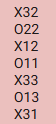
\includegraphics[width=0.22\textwidth]{images/993d0a1f141dfd79.png}\hfill
  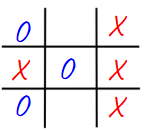
\includegraphics[width=0.28\textwidth]{images/3ece2e4bfb1630a5.png}
\end{center}
\begin{center}
\small\emph{Gauche~: capture d'écran d'un document de Soekia narrant une partie de tic-tac-toe. Droite~: une image d'une partie de tic-tac-toe où X gagne.}
\end{center}

\begin{thinkbox}
  \textbf{Y a-t-il un·e gagnant·e~?}
  \begin{itemize}
    \item Oui~! X gagne la partie.
  \end{itemize}
\end{thinkbox}

% ---------- Investigate ----------
\subsection{Exploration~: des langues artificielles}

Avez-vous remarqué que la collection de contes de fées que vous avez explorée pendant la première moitié de cette leçon n'est que l'un des nombreux corpus d'entraînement disponibles~? Explorons quelques-uns des autres.

\begin{activitybox}
  \begin{itemize}
    \item Ouvrez une fenêtre de navigateur et assurez-vous qu'elle occupe toute la largeur de votre écran.
    \item Suivez les instructions sur \emph{Qu'est-ce qui fait une langue~?} pour charger le corpus d'entraînement de tic-tac-toe dans Soekia.
    \item Complétez la première section de \emph{Qu'est-ce qui fait une langue~?}.
  \end{itemize}
\end{activitybox}

\begin{keypointbox}
  Soekia est un excellent outil pour nous permettre de regarder derrière le rideau et d'observer le traitement du langage naturel en action.

  De façon intéressante — comme le corpus de tic-tac-toe le révèle — le traitement du langage naturel ne nécessite pas réellement une langue naturelle~! (Une langue naturelle est une langue utilisée par les humains, comme l'espagnol, l'anglais ou le swahili.)

  Tout comme une langue naturelle, le texte de tic-tac-toe peut être analysé en n-grammes, puis la probabilité d'apparition de chaque n-gramme peut être déterminée. Soekia a donc pu appliquer les mêmes algorithmes que ceux utilisés sur notre corpus de contes de fées pour produire une sortie.
\end{keypointbox}

\begin{thinkbox}
  \begin{itemize}
    \item \textbf{Pouvez-vous penser à d'autres langues artificielles que Soekia pourrait être capable de traiter~?}
    \begin{itemize}
      \item Exemples possibles~: les coups d'échecs, la notation musicale.
    \end{itemize}
    \item \textbf{Qu'est-ce qui est exigé d'une langue artificielle, pour qu'elle puisse subir avec succès un traitement du langage naturel~?}
    \begin{itemize}
      \item Elle doit être découpée avec des espaces pour pouvoir être interprétée comme des «~mots~», même si elle n'est pas composée de vrais mots.
    \end{itemize}
  \end{itemize}
\end{thinkbox}

\begin{activitybox}
  \begin{itemize}
    \item Suivez les instructions de la deuxième section de \emph{Qu'est-ce qui fait une langue~?} pour accéder au corpus d'entraînement~«~Musique en notation ABC~».
    \item Complétez la deuxième section de \emph{Qu'est-ce qui fait une langue~?}, «~Penser au traitement du langage naturel~».
  \end{itemize}
\end{activitybox}

\begin{thinkbox}
  \textbf{Le traitement du langage naturel nécessite-t-il une langue naturelle~? Expliquez.}
  \begin{itemize}
    \item Non, le traitement du langage naturel fonctionne sur des langues artificielles, comme la notation des échecs et de la musique. Tant que la langue peut être découpée en «~mots~», le texte peut être traité comme une langue naturelle. Les mêmes algorithmes peuvent être appliqués à une grande variété de langues — à la fois naturelles et artificielles.
  \end{itemize}
\end{thinkbox}

% ---------- Synthesize ----------
\subsection{Synthèse}

\begin{thinkbox}
  \textbf{Un·e élève affirme que ChatGPT — qui a été construit sur le concept de la modélisation du langage — est une source d'information fiable et crédible. Comment répondriez-vous~?}
  \begin{itemize}
    \item La production que ChatGPT génère dépend du corpus sur lequel il a été entraîné.
    \item ChatGPT n'a en réalité aucun moyen d'évaluer l'exactitude et la crédibilité~; il produit simplement une sortie après l'autre en se basant sur un modèle.
    \item Le même processus qui génère du texte soi-disant «~hallucinatoire~» génère \emph{aussi} le texte «~non hallucinatoire~».
    \item L'élève qui affirme que ChatGPT est une source fiable doit comprendre que la production de ChatGPT \emph{parfois} se trouve correspondre à la réalité…~mais parfois non~!
  \end{itemize}
\end{thinkbox}

\newpage

% ===========================================================================
% ANNEXES
% ===========================================================================
\section*{Annexe A~: Fichiers du projet}

\begin{center}
\begin{tabularx}{\textwidth}{l X}
  \toprule
  \textbf{Fichier} & \textbf{Description} \\
  \midrule
  \texttt{chatbots.tex} & Document de cours (ce fichier) \\
  \texttt{famous-ai-disasters.pdf} & Polycopié optionnel~: exemples célèbres de défaillances de l'IA \\
  \texttt{images/} & 8~images~: icônes de Soekia, capture des quatre panneaux, tic-tac-toe \\
  \bottomrule
\end{tabularx}
\end{center}

\vspace{1em}
\textbf{À noter~:} cette leçon utilise l'outil \textbf{Soekia} en ligne (version française~: \url{https://www.soekia.ch/GPT/?lang=FR}), un modèle de langue statistique conçu pour l'apprentissage. Contrairement aux leçons précédentes, il n'y a pas de fichier Pyret~: toute l'exploration se fait dans l'interface web de Soekia. Le référentiel pédagogique reste le même que dans la leçon \emph{Modèles génératifs}~: un corpus est découpé en n-grammes, des probabilités sont calculées, et du texte est généré mot à mot.

\section*{Exercices supplémentaires}

\begin{itemize}
  \item \emph{Famous AI Disasters} — polycopié optionnel présentant des exemples réels d'hallucinations de l'IA (\texttt{famous-ai-disasters.pdf}).
\end{itemize}

\section*{À propos de ces supports}

Ces supports ont été développés en partie grâce au soutien de la \emph{National Science Foundation} (bourses 1042210, 1535276, 1648684, 1738598, 2031479 et 1501927).

\begin{center}
  \textbf{Bootstrap} par la Communauté Bootstrap est sous licence Creative Commons 4.0 Unported.\\
  Cette licence n'accorde pas la permission d'organiser des formations ou du développement professionnel.\\[1em]
  \textit{Traduction et adaptation française réalisées en août 2026.}\\
  \textit{Source originale~: \url{https://www.bootstrapworld.org/materials/fall2026/en-us/lessons/stat-lang-models-chatbots/}}
\end{center}

\end{document}